\section{Experimental Evaluation} \label{sec:extension_experiments}

\subsection{Overlaying Polygons with Dangle and Cut Edges}

\begin{table}
    \small
    \caption{Overlaying Polygons with Dangle and Cut Edges Dataset}
    \label{tab:dangles}
    \begin{tabular}{c c c c}
        \toprule
        Dataset & Number Layer $A$ of Polygons & Number of Layer $B$ Edges & Result Polygons \\
        \midrule
        TN & 1,272 & 3,380,780 & 41,761 \\
        GA & 1,633 & 4,647,171 & 49,125 \\
        NC & 1,272 & 7,212,604 & 22,413 \\
        TX & 4,399  & 8,682,950 & 98,635 \\
        VA & 1,554 & 8,977,361 & 38,941 \\
        CA & 7,038 & 9,103,610 & 96,916\\
        \bottomrule
    \end{tabular}
\end{table}

\begin{figure}
    \centering
    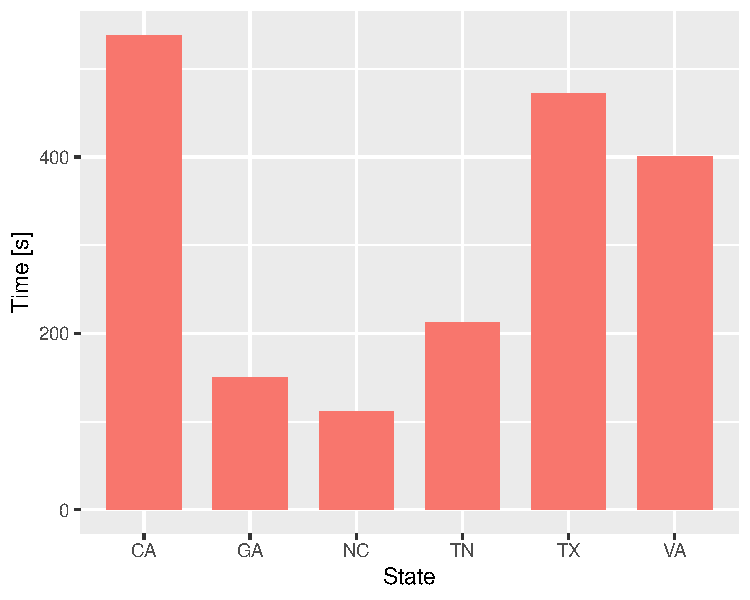
\includegraphics[width=0.75\textwidth]{chapterExtension/states.pdf}
    \caption{Overlaying State polygons with dangle and cut edges.}
    \label{fig:dangle}
\end{figure}

In this section, we examine the performance of overlaying polygons with dangle and cut edges resulting from the polygonization process, as detailed in \ref{sec:over_dang}.  Table \ref{tab:dangles} presents the number of polygons per state for the first overlay layer, the number of dangle and cut edges per state for the second overlay layer, and the number of resulting polygons per state.

From Figure \ref{fig:dangle}shows that the running time is influenced by both the number of dangle and cut edges and the number of intersections between the two layers (indicated by the number of generated polygons). TN and GA have relatively fewer dangle and cut edges, leading to lower execution times compared to VA, TX, and CA. However, because NC has significantly fewer intersections than TN and GA, it exhibits the lowest execution time overall. While TX, VA, and CA have a comparable number of edges, VA’s lower number of intersections results in a shorter execution time compared to TX and CA.
